\chapter{度量空间}
\label{chap:metric-spaces}

用有理数$1.4,1.41,1.414,\ldots$逼近$\sqrt2$时，每一项都可以说清“误差小于$10^{-n}$”；用有限个格点代表一块平面区域时，也可以说清“每一点到最近格点的距离不超过$\varepsilon$”。第~\ref{chap:topological-spaces}章的拓扑能说一列点趋于某点、一个集合在另一个中稠密，却说不出这些定量的话：它只知道哪些集合是开的，不知道误差有多大。距离补上了这一层信息。有了距离，我们还能问拓扑问不出的问题：后项彼此越来越近的点列是否一定有极限，空间在给定精度下需要多少个代表。

本章先给出度量公理，用开球生成拓扑，说明此后的开集、邻域和收敛都可以用距离判断，并讨论距离带来的有界性与可分性判据；再说明怎样由已有的距离构造子空间、乘积空间以及零距离识别后的空间。随后两节把点列放在中心：收敛等价于距离趋零，闭包由点列极限刻画；只知道点列尾部相互接近时，完备性回答极限是否存在，并给出完备化与Baire纲定理。紧性的度量判据把开覆盖条件换成收敛子列，再拆成全有界与完备两部分。最后用覆盖数、打包数和度量熵计数有限精度下所需的代表。

本章只研究单个度量空间本身。连续映射的距离判据、均匀连续、映射列的收敛和压缩迭代在第~\ref{chap:metric-space-maps}章讨论；由向量空间结构和范数产生的度量在第~\ref{chap:normed-spaces}章系统展开；函数类的覆盖估计在第~\ref{chap:function-class-covers}章进行。

\section{度量}
\label{sec:metric-metrics}

平面上两点相距多远，答案取决于怎样走。直线飞行时用欧氏距离；只能沿东西、南北两个方向分别调整、并以较慢的一个方向为准时，用两个坐标差的最大值；只关心两个位置是否相同时，相同记为$0$，不同记为$1$。本节先比较这三种规则，提炼它们共同遵守的条件，得到度量的定义；再用开球把距离变成第~\ref{chap:topological-spaces}章的拓扑，并讨论距离额外提供的有界性与可分性判据。

\subsection{度量的定义}
\label{sec:metric-definition}

取平面上两点$\bm p=(0,0)$与$\bm q=(3,4)$。三种规则给出的距离分别是
\begin{equation*}
d_2(\bm p,\bm q)=\sqrt{3^2+4^2}=5,\qquad
d_\infty(\bm p,\bm q)=\max\{3,4\}=4,\qquad
d_0(\bm p,\bm q)=1,
\end{equation*}
其中$d_2(\bm x,\bm y)=\bigl((x_1-y_1)^2+(x_2-y_2)^2\bigr)^{1/2}$，$d_\infty(\bm x,\bm y)=\max\{\lvert x_1-y_1\rvert,\lvert x_2-y_2\rvert\}$，$d_0(\bm x,\bm y)$在$\bm x=\bm y$时为$0$、否则为$1$。三个数不同，判断“谁离$\bm p$近”的结果也不同：到$\bm p$的距离小于$1$的点，在$d_2$下组成圆盘，在$d_\infty$下组成边长为$2$的正方形，在$d_0$下只有$\bm p$本身。

数值不同，三种规则却有共同之处。每个距离都不小于零，并且只有两点相同时才为零；从$\bm p$到$\bm q$与从$\bm q$到$\bm p$的距离相同；绕经第三点不会比直接比较更近。把这三条作为公理，就得到不依赖坐标的距离概念。

\begin{definition}[度量]
\label{def:metric-metric}
设$X$是非空集合。映射$d:X\times X\to[0,\infty)$若对任意$x,y,z\in X$满足
\begin{enumerate}
\item 零距离判定：$d(x,y)=0$当且仅当$x=y$；
\item 对称性：$d(x,y)=d(y,x)$；
\item 三角不等式：$d(x,z)\leq d(x,y)+d(y,z)$，
\end{enumerate}
则称$d$为$X$上的一个\term{度量}（metric），称$(X,d)$为\term{度量空间}（metric space）。
\end{definition}

非负性已经写在取值范围$[0,\infty)$里。零距离判定保证距离能区分不同的点；对称性说明距离不带方向；三角不等式说明绕道不会缩短距离，它是后面几乎所有估计的来源。度量空间由集合与度量共同确定：同一个$\mathbb R^2$配上$d_2$、$d_\infty$或$d_0$，是三个不同的度量空间，下文提到“空间$X$”时总默认已经选定了度量。

三角不等式还有一个常用的变形。对任意$x,y,z$，由$d(x,z)\leq d(x,y)+d(y,z)$得$d(x,z)-d(y,z)\leq d(x,y)$，交换$x,y$的角色又得$d(y,z)-d(x,z)\leq d(x,y)$，所以
\begin{equation}
\lvert d(x,z)-d(y,z)\rvert\leq d(x,y).
\label{eq:metric-reverse-triangle}
\end{equation}
它说明：$x$移动多少，$x$到固定点$z$的距离至多变化多少。第~\ref{chap:metric-space-maps}章用它证明距离函数连续。

\begin{example}[三种平面距离的核对]
\label{ex:metric-three-metrics}
对$d_\infty$，前两条公理直接成立。三角不等式逐坐标核对：$\lvert x_i-z_i\rvert\leq\lvert x_i-y_i\rvert+\lvert y_i-z_i\rvert\leq d_\infty(\bm x,\bm y)+d_\infty(\bm y,\bm z)$对$i=1,2$都成立，再对$i$取最大值即可。对$d_0$，若$\bm x\neq\bm z$，则$\bm y$至少与其中一点不同，右端至少为$1$；若$\bm x=\bm z$，左端为$0$。欧氏距离$d_2(\bm x,\bm y)=\lVert\bm x-\bm y\rVert_2$的三角不等式就是欧氏范数的Minkowski不等式。更一般地，任意向量空间上的范数$\lVert\cdot\rVert$都给出度量$d(\bm x,\bm y)=\lVert\bm x-\bm y\rVert$；有限维情形的范数及其三角不等式可参考\BookChapterRef{chap:normed-inner-product-spaces}{卷二“赋范空间与内积空间”章}，一般赋范空间在第~\ref{chap:normed-spaces}章讨论。
\end{example}

度量的对象不必是数或向量。设$X=\{0,1\}^n$是长度为$n$的二进制串，$d_H(x,y)$记$x,y$取值不同的位置个数，称为\term{Hamming距离}（Hamming distance）。例如$d_H(0110,0011)=2$。若$x,z$在某个位置不同，则$y$在这个位置至少与$x,z$之一不同，所以$x,z$的每个不同位置都至少计入$d_H(x,y)$与$d_H(y,z)$中的一个，三角不等式成立。

并不是每个看起来合理的“差异量”都是度量。在$\mathbb R$上取$e(x,y)=(x-y)^2$，前两条公理成立，但$e(0,2)=4$，而$e(0,1)+e(1,2)=2$，三角不等式失败。平方误差放大了大的差异，经由中间点分两步走反而“更近”；这正是它不能直接当作距离使用的原因，而它的平方根$\lvert x-y\rvert$是度量。

\subsection{度量拓扑}
\label{sec:metric-topology}

有了距离，“$x$附近”最自然的含义是距离$x$小于某个正数的那些点。我们先给这类集合命名，再说明它们怎样生成第~\ref{chap:topological-spaces}章意义下的拓扑。

\begin{definition}[开球与闭球]
\label{def:metric-balls}
设$(X,d)$是度量空间，$x\in X$。对$r>0$，称
\begin{equation*}
B(x,r)=\{y\in X:d(x,y)<r\},\qquad B[x,r]=\{y\in X:d(x,y)\leq r\}
\end{equation*}
分别为以$x$为中心、$r$为半径的\term{开球}（open ball）与\term{闭球}（closed ball）。需要指明度量时写作$B_d(x,r)$。
\end{definition}

方括号提示闭球包含距离恰为$r$的点。闭球不一定是开球的闭包：在离散度量$d_0$下，$B(x,1)=\{x\}$，它的闭包仍是$\{x\}$，而$B[x,1]$是整个空间。所以本书不用$\overline{B(x,r)}$表示闭球。

开球的关键性质是：球内每一点都被一个更小的球包在球内。

\begin{lemma}[开球内的小球]
\label{lem:metric-ball-inside-ball}
若$y\in B(x,r)$，令$s=r-d(x,y)>0$，则$B(y,s)\subseteq B(x,r)$。
\end{lemma}

\begin{proof}
对$z\in B(y,s)$，由三角不等式，$d(x,z)\leq d(x,y)+d(y,z)<d(x,y)+s=r$，所以$z\in B(x,r)$。
\end{proof}

\begin{theorem}[开球构成拓扑基]
\label{thm:metric-balls-base}
度量空间$(X,d)$中全体开球构成$X$上某个拓扑的基。由这个基生成的拓扑中，$U\subseteq X$是开集当且仅当对每个$x\in U$都存在$r>0$使$B(x,r)\subseteq U$。
\end{theorem}

\begin{proof}
按第~\ref{chap:topological-spaces}章拓扑基的判定，要核对两件事。第一，每个$x$都属于开球$B(x,1)$，所以开球覆盖$X$。第二，设$z\in B(x_1,r_1)\cap B(x_2,r_2)$，由引理~\ref{lem:metric-ball-inside-ball}，取$s=\min\{r_1-d(x_1,z),r_2-d(x_2,z)\}>0$，则$B(z,s)$同时含于两个球，因而含于它们的交。

由基生成的开集是若干基元素的并。若$U$是开球之并，$x\in U$落在某个$B(y,t)\subseteq U$中，引理~\ref{lem:metric-ball-inside-ball}给出以$x$为中心、含于$B(y,t)$的球。反过来，若每个$x\in U$都有$B(x,r_x)\subseteq U$，则$U=\bigcup_{x\in U}B(x,r_x)$是开球之并。
\end{proof}

由开球生成的拓扑称为$d$的\term{度量拓扑}（metric topology）。今后说度量空间中的开集、闭集、邻域、收敛与连续，都指这个拓扑下第~\ref{chap:topological-spaces}章的概念。按定理~\ref{thm:metric-balls-base}，集合$N$是$x$的邻域当且仅当它包含某个开球$B(x,r)$；于是$B(x,1/n)$，$n=1,2,\ldots$，构成$x$的一个可数邻域基，因为任何$B(x,r)$都包含$n>1/r$时的$B(x,1/n)$。

\paragraph{点的分离}
距离为正的两点可以用半径为距离一半的球分开。设$x\neq y$，$r=d(x,y)/2>0$。若$z\in B(x,r)\cap B(y,r)$，则$d(x,y)\leq d(x,z)+d(z,y)<2r=d(x,y)$，矛盾，所以$B(x,r)$与$B(y,r)$不交。这说明度量拓扑满足Hausdorff条件：不同的点有不交的邻域。

这条性质给出一个限制：并非每个拓扑都来自某个度量。两点集$\{a,b\}$上的平凡拓扑只有$\varnothing$和全集两个开集，$a,b$无法用不交的开集分开，所以任何度量都不能诱导它。另一个直接推论是单点集是闭集：对$y\neq x$，球$B(y,d(x,y))$不含$x$，所以$X\setminus\{x\}$是开集。

\paragraph{用球判断子集的位置}
把第~\ref{chap:topological-spaces}章的定义换成球的语言，子集$A\subseteq X$与点$x$的关系可以这样判断：$x$是$A$的内点，当且仅当某个$B(x,r)\subseteq A$；$x$属于$A$的闭包，当且仅当每个$B(x,r)$都与$A$相交；$x$属于$A$的边界，当且仅当每个$B(x,r)$既与$A$相交、又与$X\setminus A$相交。这三条都由“开球构成邻域基”直接得到。

闭球是闭集。若$d(x,y)>r$，令$s=d(x,y)-r$，对$z\in B(y,s)$有$d(x,z)\geq d(x,y)-d(y,z)>r$，所以$B(y,s)$落在$B[x,r]$的补集中，补集是开集。

\begin{example}[开闭性与边界的判断]
\label{ex:metric-open-closed-interval}
在$\mathbb R$的通常度量$\lvert x-y\rvert$下考察$A=[0,1)$。点$0$的每个球都含有负数，所以$0$不是内点，$A$不是开集；点$1$的每个球都含有$A$中的点，$1$在闭包中却不在$A$中，所以$A$也不是闭集。按上面的判据，$A$的内部为$(0,1)$，闭包为$[0,1]$，边界为$\{0,1\}$。

换成离散度量$d_0$，每个单点集都是开球$B(x,1/2)$，于是任意子集都是开集，它的补集也是开集，所以任意子集同时是开集和闭集，边界总是空集。同一个集合$[0,1)$在两种度量下开闭性不同，再次说明开闭性取决于所选的度量。
\end{example}

不同的度量也可能给出相同的拓扑。在$\mathbb R^2$中，对任意$\bm x$和$r>0$，
\begin{equation*}
B_{d_\infty}(\bm x,r/\sqrt2)\subseteq B_{d_2}(\bm x,r)\subseteq B_{d_\infty}(\bm x,r),
\end{equation*}
这由$d_\infty\leq d_2\leq\sqrt2\,d_\infty$得到。于是一种度量下的每个球内都含有另一种度量下同心的球，按定理~\ref{thm:metric-balls-base}，两者的开集完全相同。离散度量$d_0$则给出不同的拓扑：单点集在$d_0$下是开集，在$d_2$下不是。什么时候两个度量“一样好”，取决于要保留开集、柯西列还是误差尺度，第~\ref{chap:metric-space-maps}章分别讨论。

\subsection{有界集}
\label{sec:metric-bounded}

拓扑只告诉我们哪些点“附近”，不告诉我们一个集合整体有多大。距离可以回答后一个问题：一个集合能否被某个有限半径的球装下。

\begin{definition}[有界集与直径]
\label{def:metric-bounded}
度量空间$(X,d)$的子集$A$若满足：存在$x\in X$和$r>0$使$A\subseteq B(x,r)$，则称$A$为\term{有界集}（bounded set）。非空集合$A$的\term{直径}（diameter）定义为$\operatorname{diam}A=\sup\{d(a,b):a,b\in A\}\in[0,\infty]$。空集规定为有界。
\end{definition}

球心的选取并不重要。若$A\subseteq B(x,r)$，对任意$y\in X$和$a\in A$，有$d(y,a)\leq d(y,x)+d(x,a)<d(y,x)+r$，所以$A\subseteq B(y,r+d(x,y))$：换一个球心，只需把半径加上两个球心的距离。同样的估计说明，非空集合有界当且仅当它的直径有限：若$A\subseteq B(x,r)$，则$d(a,b)\leq d(a,x)+d(x,b)<2r$；反过来，若$\operatorname{diam}A<\infty$，任取$a_0\in A$，就有$A\subseteq B(a_0,\operatorname{diam}A+1)$。

有界性与开闭性互不决定。在$\mathbb R$中，$(0,1)$有界且是开集；整数集$\mathbb Z$是闭集，因为它的补集是开区间之并，但它不能被任何有限半径的球容纳；$[0,1]$既有界又闭。可见判断一个集合“大小有限”，不能从它是否包含边界点来推断。

有界性还依赖于度量，而不只依赖于拓扑。在度量空间$(X,d)$上令$d'(x,y)=\min\{d(x,y),1\}$。前两条公理显然成立；对三角不等式，若$d(x,y)\geq1$或$d(y,z)\geq1$，右端至少为$1$，不小于左端；否则右端等于$d(x,y)+d(y,z)\geq d(x,z)\geq d'(x,z)$。半径小于$1$的球在$d$和$d'$下完全相同，所以两者拓扑相同，但在$d'$下每个集合都含于$B_{d'}(x,2)$，整个$\mathbb R$也成了有界集。

\subsection{可分性的判据}
\label{sec:metric-separability}

第~\ref{chap:topological-spaces}章区分了两种可数性：局部上，每个点有可数邻域基；整体上，整个空间有可数拓扑基。还定义了可分性：存在可数的稠密子集。在度量空间中，前一种总是成立，后两种恰好等价。

局部可数性已经在第~\ref{sec:metric-topology}小节得到：$\{B(x,1/n)\}_{n\geq1}$是$x$的邻域基。但这不能推出整个空间有可数拓扑基，因为每个点各自的可数个球合起来，在点数不可数时就不再可数。$\mathbb R$配上离散度量$d_0$就是例子：每个单点集$\{x\}=B(x,1/2)$都是开集，任何拓扑基必须为每个$x$提供一个含$x$且含于$\{x\}$的基元素，即$\{x\}$本身，所以拓扑基至少有不可数个元素。

\begin{theorem}[度量空间的可分性]
\label{thm:metric-separable-second-countable}
度量空间$(X,d)$可分，当且仅当它有可数拓扑基。
\end{theorem}

\begin{proof}
先设$D\subseteq X$可数且稠密。考虑族$\mathcal B=\{B(q,r):q\in D,\ r\in\mathbb Q,\ r>0\}$，它由两个可数集的乘积编号，所以可数。设$U$是开集，$x\in U$，取$r>0$使$B(x,r)\subseteq U$，再取有理数$s$满足$0<s<r/2$。由稠密性，开球$B(x,s)$含有某个$q\in D$。于是$x\in B(q,s)$，并且对$z\in B(q,s)$有$d(x,z)\leq d(x,q)+d(q,z)<2s<r$，即$B(q,s)\subseteq B(x,r)\subseteq U$。所以每个开集都是$\mathcal B$中元素之并，$\mathcal B$是拓扑基。

反过来，设$\{U_k\}_{k\geq1}$是可数拓扑基。对每个非空的$U_k$取一点$x_k\in U_k$，令$D$为这些点组成的集合，它可数。任意非空开集$V$是基元素之并，所以包含某个非空的$U_k$，从而含有$x_k\in D$。每个非空开集都与$D$相交，$D$稠密。
\end{proof}

证明的第一步用有理半径，是为了让球的总数可数；第二步只是从每个基元素中选一个代表点。在一般拓扑空间中，第二步仍然成立，即有可数基的空间可分；第一步却用到了距离和三角不等式，一般拓扑空间中可分不保证有可数基。

\begin{example}[欧氏空间的可数基]
\label{ex:metric-rn-separable}
在$(\mathbb R^n,d_2)$中，有理坐标点集$\mathbb Q^n$可数。给定$\bm x$和$\varepsilon>0$，逐个坐标取有理数$q_i$使$\lvert x_i-q_i\rvert<\varepsilon/\sqrt n$，则$d_2(\bm x,\bm q)<\varepsilon$，所以$\mathbb Q^n$稠密。按定理~\ref{thm:metric-separable-second-countable}，以有理坐标点为中心、有理数为半径的球构成可数拓扑基。前面的离散$\mathbb R$没有可数基，相应地它也不可分：每个单点集都是开集，稠密子集必须与每个单点集相交，只能是$\mathbb R$本身。
\end{example}

这个等价关系还有一个推论：可分度量空间的每个子集，按限制下来的度量也可分。原因是可数拓扑基$\{U_k\}$与子集$A$的交$\{U_k\cap A\}$构成$A$的可数拓扑基；这里用到子集上的拓扑恰是限制度量给出的拓扑，第~\ref{sec:metric-subspace}小节会证明这一点。例如$\mathbb R^2$中的任意曲线都可分，推论直接给出这一点，不需要具体找出它的可数稠密子集；对无理数集，也可以直接核对$\{q+\sqrt2:q\in\mathbb Q\}$是它的可数稠密子集。

\section{度量的构造}
\label{sec:metric-constructions}

第~\ref{chap:topological-spaces}章从已有空间构造了子空间、有限乘积和商空间，每次都规定了新空间的开集。有了距离以后，我们希望直接写出新空间的距离，并且让它诱导的拓扑恰好就是那里规定的拓扑。

本节逐项核对三种构造：把距离限制到子集，把各坐标的距离组合起来，以及先允许不同的点距离为零、再把这些点识别为一点。前两种对任意度量空间都可行；第三种只适用于由距离本身决定的识别，不能推广为任意商空间都有度量。

\subsection{子空间}
\label{sec:metric-subspace}

研究度量空间的一部分时，最直接的做法是保留原来的两点距离，只限制允许出现的点。

\begin{definition}[子空间度量]
\label{def:metric-subspace-metric}
设$(X,d)$是度量空间，$A\subseteq X$非空。限制$d_A=d|_{A\times A}$称为$A$上的\term{子空间度量}（subspace metric），$(A,d_A)$称为$X$的度量子空间。
\end{definition}

$A$中的点仍是$X$中的点，三条公理对$X$中任意点成立，自然对$A$中的点成立，所以$d_A$是度量。需要核对的是拓扑。$d_A$的开球是
\[
B_A(a,r)=\{y\in A:d(a,y)<r\}=B(a,r)\cap A,
\]
也就是环境中的球与$A$的交。

\begin{theorem}[子空间度量的拓扑]
\label{thm:metric-subspace-topology}
$d_A$诱导的拓扑等于$A$从$X$继承的子空间拓扑，即$V\subseteq A$在$(A,d_A)$中是开集，当且仅当存在$X$的开集$U$使$V=U\cap A$。
\end{theorem}

\begin{proof}
设$V$在$(A,d_A)$中是开集。对每个$a\in V$取$r_a>0$使$B_A(a,r_a)\subseteq V$，令$U=\bigcup_{a\in V}B(a,r_a)$。它是$X$的开集，并且
\[
U\cap A=\bigcup_{a\in V}\bigl(B(a,r_a)\cap A\bigr)=\bigcup_{a\in V}B_A(a,r_a)=V.
\]

反过来，设$U$是$X$的开集，$a\in U\cap A$。取$r>0$使$B(a,r)\subseteq U$，则$B_A(a,r)=B(a,r)\cap A\subseteq U\cap A$，所以$U\cap A$在$(A,d_A)$中是开集。
\end{proof}

于是第~\ref{chap:topological-spaces}章关于子空间的结论在度量子空间中都可以直接使用，只是开闭性要相对于$A$来判断。图~\ref{fig:metric-subspace-chord-arc}(a)是一个例子：在$\mathbb R$中取$A=[0,1]$，以$0$为中心、半径$1/2$的球在$A$中只剩$[0,1/2)$。

\begin{BookInlineFigure}
  \centering
  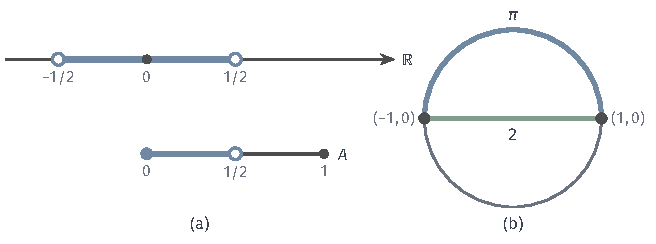
\includegraphics[width=111.1mm]{figures/04-spaces-measures-and-geometry/01-topology-and-metric/tikz/metric-subspace-chord-arc/figure.pdf}
  \caption{子空间的两个特点。(a)实轴上以$0$为中心、半径$1/2$的开球是$(-1/2,1/2)$，限制到$A=[0,1]$后成为$[0,1/2)$，它在$A$中是开集，在$\mathbb R$中不是。(b)单位圆周上，子空间度量量的是绿色弦长$2$，沿圆周的最短路径是蓝色半圆，长度$\pi$。}
  \label{fig:metric-subspace-chord-arc}
\end{BookInlineFigure}

这个集合可以写成$[0,1/2)=(-1/2,1/2)\cap A$，所以在$A$中是开集；$0$的左侧没有$A$的点，也就没有“越界”的点来破坏开性。再取$A=(0,1]$，它作为自身的子集总是闭集，但它在$\mathbb R$中不是闭集。环境决定了哪些点可以用来检验开闭。

子空间只保留环境中的两点距离，并不改用“沿着子集走”的距离。设$S^1=\{\bm x\in\mathbb R^2:\lVert\bm x\rVert_2=1\}$是单位圆周，如图~\ref{fig:metric-subspace-chord-arc}(b)所示，子空间度量下$(1,0)$与$(-1,0)$的距离是弦长$2$，而沿圆周走的最短长度是$\pi$。

弧长是圆周上另一个度量，它与弦长度量给出同样的拓扑，数值却不同。沿曲面或流形内部量出的路径长度需要切向量与长度的概念，在第~\ref{chap:riemannian-geometry}章建立。

\subsection{有限乘积空间}
\label{sec:metric-product}

几个度量空间的点组成坐标组时，需要一个距离同时比较各个坐标。设$(X_1,d_1),\ldots,(X_m,d_m)$是度量空间，$X=X_1\times\cdots\times X_m$，点记作$x=(x_1,\ldots,x_m)$。最常用的两种组合方式是求和与取最大：
\begin{equation}
\rho_1(x,y)=\sum_{i=1}^m d_i(x_i,y_i),\qquad
\rho_\infty(x,y)=\max_{1\leq i\leq m}d_i(x_i,y_i).
\label{eq:metric-product-metrics}
\end{equation}
这样定义的距离称为\term{乘积度量}（product metric）。$\mathbb R^2$上的$d_\infty$就是两个实轴的$\rho_\infty$。

两者都是度量。和或最大值为零，当且仅当每个$d_i(x_i,y_i)=0$，即每个坐标相同，这给出零距离判定；对称性逐坐标成立。三角不等式从每个坐标的不等式出发：
\[
d_i(x_i,z_i)\leq d_i(x_i,y_i)+d_i(y_i,z_i).
\]
对$\rho_1$，把这些不等式逐项相加。对$\rho_\infty$，右端两项分别不超过$\rho_\infty(x,y)$与$\rho_\infty(y,z)$，再对$i$取最大值。

两种度量还满足
\[
\rho_\infty\leq\rho_1\leq m\,\rho_\infty,
\]
因为$m$个非负数的和不小于其中最大的一个，也不超过最大者的$m$倍。图~\ref{fig:metric-ball-nesting}(b)画出了$m=2$时这组不等式对应的球的嵌套。与第~\ref{sec:metric-topology}小节的平面情形一样，它们的开球互相嵌套，诱导相同的拓扑。

\begin{theorem}[乘积度量的拓扑]
\label{thm:metric-product-topology}
$\rho_1$与$\rho_\infty$诱导的拓扑都等于第~\ref{chap:topological-spaces}章中$X_1,\ldots,X_m$的有限乘积拓扑。
\end{theorem}

\begin{proof}
由于两者诱导相同的拓扑，只需对$\rho_\infty$证明。乘积拓扑以形如$U_1\times\cdots\times U_m$（每个$U_i$是$X_i$的开集）的集合为基。最大值小于$r$等价于每个坐标距离都小于$r$，所以$\rho_\infty$的开球恰是
\[
B_{\rho_\infty}(x,r)=B_{d_1}(x_1,r)\times\cdots\times B_{d_m}(x_m,r).
\]
每个开球都是乘积拓扑的基元素，度量拓扑的开集都是乘积拓扑的开集。

反过来，设$x\in U_1\times\cdots\times U_m$。对每个$i$取$r_i>0$使$B_{d_i}(x_i,r_i)\subseteq U_i$，令$r=\min_i r_i$，则$B_{\rho_\infty}(x,r)\subseteq U_1\times\cdots\times U_m$。所以乘积拓扑的基元素在度量拓扑中也是开集。
\end{proof}

\begin{example}[两类坐标的乘积]
\label{ex:metric-product-two-coordinates}
取$X_1=\mathbb R$（通常距离）与$X_2=\{0,1\}^3$（Hamming距离），点$x=(0.2,010)$、$y=(0.5,011)$。实数坐标相差$0.3$，二进制串相差$1$位，于是
\[
\rho_1(x,y)=0.3+1=1.3,\qquad\rho_\infty(x,y)=\max\{0.3,1\}=1.
\]

在$\rho_\infty$下，$x$的半径$1/2$的球由第二坐标与$010$相同、第一坐标落在$(-0.3,0.7)$中的点组成：Hamming距离只取整数，要求它小于$1/2$就是要求两个串完全相同。
\end{example}

可见乘积距离小，意味着每个坐标都必须接近；哪个坐标先限制住球的形状，取决于各坐标距离的取值方式。

\subsection{伪度量}
\label{sec:metric-pseudometric}

有时我们只通过某些特征比较对象。比较平面上的点时如果只看横坐标，令
\begin{equation}
p(\bm x,\bm y)=\lvert x_1-y_1\rvert,
\label{eq:metric-first-coordinate-pseudometric}
\end{equation}
则$(0,0)$与$(0,5)$的“距离”为零，尽管它们是不同的点。$p$满足对称性和三角不等式，也满足$p(\bm x,\bm x)=0$，只缺零距离判定中“距离为零推出两点相同”这一半。

\begin{definition}[伪度量]
\label{def:metric-pseudometric}
设$X$非空。映射$p:X\times X\to[0,\infty)$若对任意$x,y,z\in X$满足$p(x,x)=0$、$p(x,y)=p(y,x)$与$p(x,z)\leq p(x,y)+p(y,z)$，则称$p$为$X$上的\term{伪度量}（pseudometric）。
\end{definition}

伪度量常由“忽略一部分信息”产生。向量空间上的\term{半范数}（seminorm）$\lVert\cdot\rVert$允许非零向量的长度为零，$p(\bm x,\bm y)=\lVert\bm x-\bm y\rVert$就是伪度量。第~\ref{chap:integration}章用积分比较函数时会遇到同样的情形：两个只在一个点上取值不同的函数，按积分算出的差异为零。

伪度量仍然有开球$B_p(x,r)=\{y:p(x,y)<r\}$。第~\ref{sec:metric-topology}小节证明开球构成拓扑基时，只用了“每点到自身距离为零”（使$x\in B(x,r)$）与三角不等式，没有用到“距离为零推出两点相同”。所以那里的论证逐字适用：伪度量的开球也生成一个拓扑，开集的球判据也相同。

这个拓扑不能区分零距离的点。在横坐标伪度量下，开球是一条竖直带形：
\[
B_p((0,0),1)=\{\bm x:\lvert x_1\rvert<1\},
\]
它同时包含$(0,0)$与$(0,5)$，见图~\ref{fig:metric-pseudometric-quotient}。一般地，若$p(x,y)=0$，则对任意$r>0$有$y\in B_p(x,r)$且$x\in B_p(y,r)$，于是$x$的每个开邻域都含有$y$，反之亦然。

所以只要存在不同的零距离点，伪度量拓扑就不满足Hausdorff条件。极限也随之不唯一：常值点列$(0,0),(0,0),\ldots$按$p$既趋于$(0,0)$，也趋于$(0,5)$。

\begin{BookInlineFigure}
  \centering
  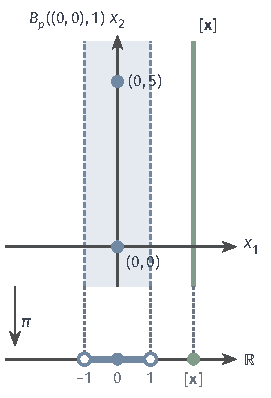
\includegraphics[width=45.903mm]{figures/04-spaces-measures-and-geometry/01-topology-and-metric/tikz/metric-pseudometric-quotient/figure.pdf}
  \caption{横坐标伪度量及其等价类。蓝色竖直带形是开球$B_p((0,0),1)$，点$(0,0)$与$(0,5)$同在其中，无法区分。绿色竖线是一个等价类$[\bm x]$。商映射$\pi$把每条竖线压成实轴上的一点，带形压成开区间$(-1,1)$。}
  \label{fig:metric-pseudometric-quotient}
\end{BookInlineFigure}

\subsection{零距离等价类上的度量}
\label{sec:metric-quotient}

既然伪度量无法区分零距离的点，自然的做法是把它们当成同一个点。下面验证这样做的每一步都合理，并说明得到的空间就是第~\ref{chap:topological-spaces}章意义下的商空间。

设$p$是$X$上的伪度量。规定$x\sim y$当且仅当$p(x,y)=0$。它是等价关系：自反性来自$p(x,x)=0$，对称性来自$p$的对称性，传递性来自
\[
p(x,z)\leq p(x,y)+p(y,z)=0.
\]
记$x$的等价类为$[x]$，商集为$X/{\sim}$，商映射为$\pi(x)=[x]$。

\begin{theorem}[零距离等价类上的度量]
\label{thm:metric-quotient-metric}
令$\hat d([x],[y])=p(x,y)$。则$\hat d$不依赖代表元的选取，是$X/{\sim}$上的度量，并且它诱导的拓扑等于$\pi$给出的商拓扑。
\end{theorem}

\begin{proof}
先证$\hat d$定义合理。设$x\sim x'$，$y\sim y'$。式~\eqref{eq:metric-reverse-triangle}的推导只用了对称性与三角不等式，所以对$p$也成立。于是
\[
\begin{aligned}
\lvert p(x,y)-p(x',y')\rvert
&\leq\lvert p(x,y)-p(x',y)\rvert+\lvert p(x',y)-p(x',y')\rvert\\
&\leq p(x,x')+p(y,y')=0.
\end{aligned}
\]

再核对公理。对称性与三角不等式从$p$继承。若$\hat d([x],[y])=0$，则$p(x,y)=0$，即$[x]=[y]$，零距离判定成立。

最后比较拓扑。由定义，$\pi$把$B_p(x,r)$映成$B_{\hat d}([x],r)$，并且
\[
\pi^{-1}\bigl(B_{\hat d}([x],r)\bigr)=B_p(x,r).
\]

设$V$在$\hat d$下是开集，$x\in\pi^{-1}(V)$。取$r$使$B_{\hat d}([x],r)\subseteq V$，则$B_p(x,r)\subseteq\pi^{-1}(V)$，所以$\pi^{-1}(V)$是$p$下的开集，$V$是商拓扑的开集。

反过来，设$\pi^{-1}(V)$是开集，$[x]\in V$。取$r$使$B_p(x,r)\subseteq\pi^{-1}(V)$，则$B_{\hat d}([x],r)=\pi(B_p(x,r))\subseteq V$，所以$V$在$\hat d$下是开集。
\end{proof}

回到横坐标伪度量。$(x_1,x_2)$的等价类是竖直线$\{x_1\}\times\mathbb R$，映射$[\bm x]\mapsto x_1$是$X/{\sim}$到$\mathbb R$的双射，并且
\[
\hat d([\bm x],[\bm y])=\lvert x_1-y_1\rvert.
\]
所以把零距离的点识别以后，得到的正是带通常距离的实轴：竖直方向的信息被丢掉，横坐标的距离被完整保留，这就是图~\ref{fig:metric-pseudometric-quotient}中从上到下的投影。

这一构造之所以可行，是因为等价关系由$p$自身给出，球在识别前后一一对应。对任意等价关系，商空间未必有度量。在$\mathbb R$上规定$x\approx y$当且仅当$x-y\in\mathbb Q$，考察商拓扑中的非空开集$U$。

$U$在$\mathbb R$中的原像是非空开集，含有某个区间$(a,b)$，又是若干等价类之并，因而含有$(a,b)+\mathbb Q=\mathbb R$。于是商拓扑只有空集和全集两个开集。商集有无穷多个点，两个不同的点不能用不交开集分开，按第~\ref{sec:metric-topology}小节的分离性，任何度量都不能诱导这个拓扑。

\section{点列收敛}
\label{sec:metric-convergence}

第~\ref{chap:topological-spaces}章用邻域定义收敛：$x_n\to x$是指$x$的每个邻域都包含点列中除有限项以外的全部项。这个定义要求逐个检查邻域，在度量空间中可以换成一个实数列的极限。

本节先证明这一点，再整理收敛点列的基本性质，并给出闭包、稠密与闭集的序列判据。序列判据的反向部分依赖“每点有可数个球作邻域基”，所以不能无条件搬到一般拓扑空间。

\begin{theorem}[收敛的距离判据]
\label{thm:metric-convergence-distance}
在度量空间$(X,d)$中，$x_n\to x$当且仅当实数列$d(x_n,x)\to0$。
\end{theorem}

\begin{proof}
设$x_n\to x$。对$\varepsilon>0$，$B(x,\varepsilon)$是$x$的邻域，所以存在$N$使$n\geq N$时$x_n\in B(x,\varepsilon)$，即$d(x_n,x)<\varepsilon$。

反过来，设$d(x_n,x)\to0$，$U$是$x$的邻域。按第~\ref{sec:metric-topology}小节，$U$包含某个$B(x,r)$。取$N$使$n\geq N$时$d(x_n,x)<r$，这些项就都落在$U$中。
\end{proof}

这个判据把点在空间中的运动压缩成一列实数。例如取平面点列
\[
x_n=\Bigl(\frac{\cos n}{n},\frac{\sin n}{n}\Bigr),
\]
它绕着原点$x$转圈，看上去方向杂乱，但到原点的距离恰为$d_2(x_n,x)=1/n$，由定理~\ref{thm:metric-convergence-distance}可知$x_n\to x$。

图~\ref{fig:metric-sequence-tail}把两种读法并排放在一起。取$\varepsilon=1/5$：不等式$1/n<1/5$等价于$n>5$，所以从第$N=6$项起，点列全部落进$B(x,\varepsilon)$。

\begin{BookInlineFigure}
  \centering
  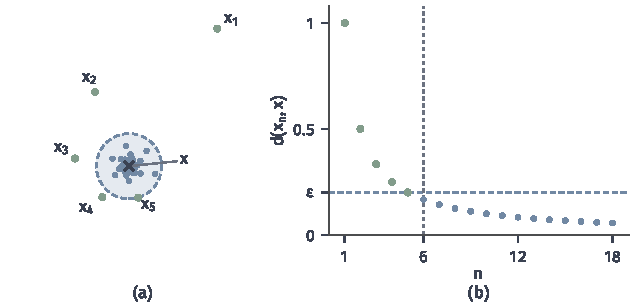
\includegraphics[width=108mm]{figures/04-spaces-measures-and-geometry/01-topology-and-metric/matplotlib/metric-sequence-tail/figure.pdf}
  \caption{点列$x_n=(\cos n/n,\sin n/n)$趋于原点$x$的两种读法，取$\varepsilon=1/5$。(a)平面上的点列，虚线圆是$B(x,\varepsilon)$，绿点是落在球外的前五项，蓝点是其后各项。(b)同一点列的距离数列$d(x_n,x)=1/n$，竖虚线处$N=6$，此后各点都在水平虚线$\varepsilon$之下。}
  \label{fig:metric-sequence-tail}
\end{BookInlineFigure}

判据的另外两个用法也值得记下。在乘积空间$(\mathbb R^m,\rho_\infty)$中，$\rho_\infty(\bm x_n,\bm x)\to0$当且仅当每个坐标的误差都趋于零，所以收敛就是逐坐标收敛；由于$\rho_1$与$\rho_\infty$诱导相同拓扑，换用$\rho_1$结论不变。

在离散度量$d_0$下，$d_0(x_n,x)$只取$0$和$1$，趋于零意味着从某项起恒为零。所以离散空间中的收敛点列，必须从某项起恒等于极限。

\subsection{收敛点列的性质}
\label{sec:metric-convergent-properties}

距离给出的第一个推论是极限唯一。若$x_n\to x$且$x_n\to y$，由三角不等式
\[
d(x,y)\leq d(x,x_n)+d(x_n,y)\to0,
\]
所以$d(x,y)=0$，由零距离判定得$x=y$。这里起作用的正是度量区分不同点的能力；第~\ref{sec:metric-pseudometric}小节的伪度量缺少这一条，常值点列可以同时趋于两个不同的点。

\begin{theorem}[收敛点列有界]
\label{thm:metric-convergent-bounded}
度量空间中的收敛点列，其全部项组成的集合是有界集。
\end{theorem}

\begin{proof}
设$x_n\to x$。取$N$使$n\geq N$时$d(x_n,x)<1$，前面只剩有限项，取它们的距离的最大值：
\[
r=1+\max\{d(x_1,x),\ldots,d(x_{N-1},x)\}
\]
（$N=1$时取$r=1$）。于是对每个$n$都有$d(x_n,x)<r$，全部项落在$B(x,r)$中。
\end{proof}

研究不收敛的点列时，常常从中挑出一部分。设$n_1<n_2<\cdots$是严格递增的正整数列，称$(x_{n_k})_{k\geq1}$为$(x_n)$的一个\term{子列}（subsequence）。严格递增保证$n_k\geq k$，所以$k\to\infty$时$n_k\to\infty$。

收敛点列的每个子列都收敛到同一个极限。设$x_n\to x$，对$\varepsilon>0$取$N$使$n\geq N$时$d(x_n,x)<\varepsilon$。当$k\geq N$时$n_k\geq N$，于是$d(x_{n_k},x)<\varepsilon$。

反方向不成立：一个点列有收敛的子列，不能推出它本身收敛。在$\mathbb R$中取$x_n=(-1)^n$，偶数项组成的子列恒为$1$，奇数项组成的子列恒为$-1$，各自收敛。若整列趋于某个$x$，两个子列都应趋于$x$，于是$x=1=-1$，矛盾。

整列收敛是比“存在收敛子列”强得多的要求，第~\ref{sec:metric-compactness}节的紧性判据只要求后者。

\subsection{闭包与闭集的序列判据}
\label{sec:metric-closure-sequences}

一个点离一个集合多近，可以用它到集合中各点距离的下确界来衡量。

\begin{definition}[点到集合的距离]
\label{def:metric-point-set-distance}
设$A\subseteq X$非空，$x\in X$。称
\begin{equation}
d(x,A)=\inf_{a\in A}d(x,a)
\label{eq:metric-point-set-distance}
\end{equation}
为$x$到$A$的\term{点到集合的距离}（distance from a point to a set）。
\end{definition}

在$\mathbb R$中取$A=(0,1)$，从定义算出
\[
d(2,A)=1,\qquad d(1,A)=0.
\]
第二个结果说明，下确界为零并不意味着$x\in A$，只说明$A$中有任意接近$x$的点。这正是闭包描述的情形。

\begin{theorem}[闭包的序列判据]
\label{thm:metric-closure-sequential}
设$A\subseteq X$非空，$x\in X$。以下三条等价：
\begin{enumerate}
\item $d(x,A)=0$；
\item $x$属于$A$的闭包$\overline A$；
\item 存在$A$中的点列$(a_n)$使$a_n\to x$。
\end{enumerate}
\end{theorem}

\begin{proof}
由(1)推(3)。对每个$n$，下确界为零意味着存在$a_n\in A$使$d(x,a_n)<1/n$，于是$a_n\to x$。

由(3)推(2)。$x$的每个邻域都包含某个$B(x,r)$，而$n$充分大时$a_n\in B(x,r)$，所以每个邻域都与$A$相交。

由(2)推(1)。对每个$n$，$B(x,1/n)$与$A$相交，取其中一点$a$，得$d(x,A)\leq d(x,a)<1/n$。$n$任意，所以$d(x,A)=0$。
\end{proof}

证明中由(1)推(3)的一步对每个$n$选出一个点，用的是可数个半径$1/n$，这正是度量空间每点有可数邻域基的用处。由(3)推(2)在任意拓扑空间中都成立，反方向则不然：第~\ref{chap:topological-spaces}章的余可数拓扑中，$\mathbb R\setminus\{0\}$的闭包是$\mathbb R$，却没有其中的点列收敛到$0$。

点到集合的距离本身也随$x$连续变化。对任意$a\in A$，由三角不等式
\[
d(x,A)\leq d(x,a)\leq d(x,y)+d(y,a).
\]
对$a$取下确界，得$d(x,A)\leq d(x,y)+d(y,A)$；交换$x,y$，又得到另一侧的不等式。合起来是
\begin{equation}
\lvert d(x,A)-d(y,A)\rvert\leq d(x,y).
\label{eq:metric-distance-to-set-lipschitz}
\end{equation}
因此闭包$\overline A=\{x:d(x,A)=0\}$可以看成一个连续函数的零点集，第~\ref{chap:metric-space-maps}章将从连续映射的角度回到这一点。

把定理~\ref{thm:metric-closure-sequential}用于两类特殊的集合，就得到稠密集和闭集的判据。$A$稠密是指$\overline A=X$，所以$A$在$X$中稠密，当且仅当$X$的每个点都是$A$中某个点列的极限。

$A$是闭集是指$\overline A=A$，所以$A$是闭集，当且仅当$A$中的点列只要在$X$中收敛，极限就属于$A$。

\begin{example}[序列判据的使用]
\label{ex:metric-sequential-criteria}
有理数在$\mathbb R$中稠密：对实数$x$，取它的十进制截断$q_n$（保留$n$位小数），则$\lvert x-q_n\rvert\leq10^{-n}$，$q_n\to x$。

集合$[0,1]$是闭集：若$a_n\in[0,1]$且$a_n\to x$，不等式在极限下保持，所以$0\leq x\leq1$。集合$(0,1]$不是$\mathbb R$的闭集：$1/n\in(0,1]$趋于$0\notin(0,1]$。

但若环境空间换成$X=(0,1]$，同一个点列在$X$中没有极限，$(0,1]$作为$X$自身仍是闭集。闭集的序列判据只要求保留环境中已经存在的极限；环境缺少某个极限点时，判据不对它提出要求。
\end{example}

环境本身是否缺少极限，正是下一节完备性要讨论的问题。

\section{完备性}
\label{sec:metric-completeness}

用迭代或截断逼近一个未知对象时，我们通常只能看到近似值本身：后面的项彼此越来越接近，极限却正是要找的东西，事先并不知道它在哪里。要判断这样的点列有没有极限，就需要一个只用点列内部距离表述的条件，这就是柯西列。本节先定义柯西列和完备空间，再讨论子空间何时完备，最后说明怎样补入缺失的极限，以及完备性带来的Baire纲定理。

\subsection{完备空间}
\label{sec:metric-complete-spaces}

收敛点列的后项不仅接近极限，也彼此接近。把后一性质单独拿出来，就得到不提及极限的条件。

\begin{definition}[柯西列]
\label{def:metric-cauchy}
度量空间$(X,d)$中的点列$(x_n)$若满足：对任意$\varepsilon>0$，存在$N$，使$m,n\geq N$时$d(x_m,x_n)<\varepsilon$，则称$(x_n)$为\term{柯西列}（Cauchy sequence）。
\end{definition}

\begin{lemma}[柯西列的基本性质]
\label{lem:metric-cauchy-basic}
在度量空间中：
\begin{enumerate}
\item 收敛点列是柯西列；
\item 柯西列是有界的；
\item 有收敛子列的柯西列本身收敛，并且收敛到该子列的极限。
\end{enumerate}
\end{lemma}

\begin{proof}
(1)设$x_n\to x$。对$\varepsilon>0$取$N$使$n\geq N$时$d(x_n,x)<\varepsilon/2$，则$m,n\geq N$时$d(x_m,x_n)\leq d(x_m,x)+d(x,x_n)<\varepsilon$。

(2)取$\varepsilon=1$对应的$N$，则$n\geq N$时$x_n\in B(x_N,1)$；前面只有有限项，按定理~\ref{thm:metric-convergent-bounded}证明中的办法放大半径即可。

(3)设$x_{n_k}\to x$。对$\varepsilon>0$，取$N$使$m,n\geq N$时$d(x_m,x_n)<\varepsilon/2$，再取$k$使$n_k\geq N$且$d(x_{n_k},x)<\varepsilon/2$。于是$n\geq N$时$d(x_n,x)\leq d(x_n,x_{n_k})+d(x_{n_k},x)<\varepsilon$。
\end{proof}

柯西列不一定收敛，关键看极限是否在当前空间中。用$\sqrt2$的十进制截断得到有理数列$q_1=1.4$，$q_2=1.41$，$q_3=1.414$，……。当$m\geq n$时$q_m$与$q_n$的前$n$位小数相同，所以$\lvert q_m-q_n\rvert<10^{-n}$，这是$\mathbb Q$中的柯西列。在$\mathbb R$中它趋于$\sqrt2$；若它在$\mathbb Q$中趋于某个有理数$q$，那么在$\mathbb R$中也趋于$q$，由极限唯一得$q=\sqrt2$，矛盾。所以这个柯西列在$\mathbb Q$中没有极限。

\begin{definition}[完备度量空间]
\label{def:metric-complete}
若度量空间$(X,d)$中的每个柯西列都在$X$中收敛，则称$(X,d)$是\term{完备度量空间}（complete metric space）。
\end{definition}

实轴是完备的：实数列收敛当且仅当它是柯西数列，这是确界原理的推论，可参考\BookChapterRef{chap:limits-continuity}{卷一“极限与连续”章}的柯西收敛准则。由此$(\mathbb R^n,\rho_\infty)$也完备：$\rho_\infty$下的柯西列在每个坐标上都是实柯西数列，各坐标分别收敛，而第~\ref{sec:metric-convergence}节说明逐坐标收敛就是$\rho_\infty$下的收敛。离散度量空间也完备：取$\varepsilon=1/2$，柯西列从某项起两两距离小于$1/2$，即从某项起恒定。

不完备的例子同样常见。$\mathbb Q$不完备，上面的截断列就是证据；区间$(0,1)$不完备，$1/(n+1)$是其中的柯西列，在$\mathbb R$中趋于$0$，但$0$不在区间内。这两个例子中的缺口性质不同：$\mathbb Q$缺少无理数，$(0,1)$只缺两个端点。完备性还依赖度量而不只依赖拓扑，第~\ref{chap:metric-space-maps}章会在实轴上构造一个与通常度量拓扑相同、却不完备的度量。

\subsection{闭子空间的完备性}
\label{sec:metric-closed-complete}

子空间是否完备，取决于它是否保留了环境中柯西列的极限。第~\ref{sec:metric-closure-sequences}小节的闭集判据正好描述这件事。

\begin{theorem}[闭子空间与完备子空间]
\label{thm:metric-closed-complete}
设$(X,d)$是度量空间，$A\subseteq X$非空。
\begin{enumerate}
\item 若$X$完备且$A$是闭集，则$(A,d_A)$完备；
\item 若$(A,d_A)$完备，则$A$是$X$的闭集，这里不要求$X$完备。
\end{enumerate}
因此在完备空间中，子空间完备当且仅当它是闭集。
\end{theorem}

\begin{proof}
(1)设$(a_n)$是$A$中的柯西列。子空间距离与环境距离相同，所以它也是$X$中的柯西列，由$X$完备收敛到某个$x\in X$。$A$是闭集，按序列判据$x\in A$，于是$(a_n)$在$A$中收敛。

(2)设$x\in\overline A$，按定理~\ref{thm:metric-closure-sequential}取$a_n\in A$使$a_n\to x$。由引理~\ref{lem:metric-cauchy-basic}，$(a_n)$是柯西列，它在完备的$A$中收敛到某个$a\in A$；在$X$中它既趋于$x$又趋于$a$，由极限唯一得$x=a\in A$。所以$\overline A=A$。
\end{proof}

在$\mathbb R$中，$[0,1]$与$\mathbb Z$都是闭集，因而完备；$\mathbb Q$不是闭集，相应地不完备。第(1)条的环境完备性不能省略。在$X=\mathbb Q$中，$A=\mathbb Q\cap[0,2]$是闭集，因为它是闭集$[0,2]$与$\mathbb Q$的交，但截断列$q_n$全在$A$中且在$A$中没有极限。同样，$A=(0,1/2]$在$X=(0,1)$中是闭集，却不完备。闭是相对于环境的性质，完备是空间自身的性质；只有当环境本身不缺极限时，前者才能保证后者。

\subsection{完备化}
\label{sec:metric-completion}

不完备的空间缺少一些极限。补入它们的思路是：既然缺失的极限只能通过柯西列来指认，就把柯西列本身当作新点；两个柯西列若彼此越来越近，它们指认的是同一个缺失点，应当识别。第~\ref{sec:metric-quotient}小节的零距离识别正好完成这一步。

设$(X,d)$是度量空间，$\mathcal C$是$X$中全体柯西列组成的集合。对$(x_n),(y_n)\in\mathcal C$，由三角不等式两次，
\begin{equation*}
\lvert d(x_n,y_n)-d(x_m,y_m)\rvert\leq d(x_n,x_m)+d(y_n,y_m),
\end{equation*}
所以$d(x_n,y_n)$是实柯西数列。实轴完备，于是可以定义
\begin{equation}
p\bigl((x_n),(y_n)\bigr)=\lim_{n\to\infty}d(x_n,y_n).
\label{eq:metric-completion-pseudometric}
\end{equation}
$p$的对称性和三角不等式由$d$逐项继承后取极限得到，$p((x_n),(x_n))=0$，所以$p$是$\mathcal C$上的伪度量。但它不是度量：$(1/n)$与$(0)$在$\mathbb R$中是不同的柯西列，$p$却为零。

按第~\ref{sec:metric-quotient}小节，把$p$为零的柯西列识别，得到度量空间$(\hat X,\hat d)$，其中$\hat X=\mathcal C/{\sim}$，$(x_n)\sim(y_n)$当且仅当$d(x_n,y_n)\to0$。对$x\in X$，令$\iota(x)$为常值点列$(x,x,\ldots)$的等价类。

\begin{theorem}[完备化]
\label{thm:metric-completion}
对任意度量空间$(X,d)$，上面构造的$(\hat X,\hat d)$是完备度量空间，$\iota:X\to\hat X$满足$\hat d(\iota(x),\iota(y))=d(x,y)$，并且$\iota(X)$在$\hat X$中稠密。
\end{theorem}

\begin{proof}
保持距离由定义直接得到：常值点列的逐项距离恒为$d(x,y)$。

稠密性：设$\xi\in\hat X$由柯西列$(x_n)$代表。对$\varepsilon>0$取$N$使$m,n\geq N$时$d(x_m,x_n)<\varepsilon$，则$m\geq N$时
\begin{equation*}
\hat d(\iota(x_m),\xi)=\lim_{n\to\infty}d(x_m,x_n)\leq\varepsilon.
\end{equation*}
所以$\iota(x_m)\to\xi$，$\xi$是$\iota(X)$中点列的极限。

完备性：设$(\xi_k)$是$\hat X$中的柯西列。由稠密性，对每个$k$取$x_k\in X$使$\hat d(\iota(x_k),\xi_k)<1/k$。由三角不等式与保持距离，
\begin{equation*}
d(x_k,x_l)=\hat d(\iota(x_k),\iota(x_l))<\tfrac1k+\hat d(\xi_k,\xi_l)+\tfrac1l,
\end{equation*}
右端在$k,l$充分大时任意小，所以$(x_k)$是$X$中的柯西列，记它的等价类为$\xi$。由稠密性证明中的估计，$\hat d(\iota(x_k),\xi)=\lim_l d(x_k,x_l)\to0$（$k\to\infty$），于是
\begin{equation*}
\hat d(\xi_k,\xi)\leq\hat d(\xi_k,\iota(x_k))+\hat d(\iota(x_k),\xi)<\tfrac1k+\hat d(\iota(x_k),\xi)\to0.
\end{equation*}
所以$\xi_k\to\xi$，$\hat X$完备。
\end{proof}

称$(\hat X,\hat d)$为$X$的\term{完备化}（completion）。保持距离的映射$\iota$让我们可以把$X$看成$\hat X$的子空间，$\hat X$中的新点恰好是$X$中柯西列的极限。若$X$本身完备，每个柯西列都等价于其极限的常值点列，$\iota$是满射，完备化不增加新点。

完备化在只差一个保持距离的双射的意义下唯一：若另有完备空间包含$X$的一个保持距离的稠密副本，它与$\hat X$之间存在保持距离的双射。证明需要把稠密子集上的映射延拓到全空间，留到第~\ref{chap:metric-space-maps}章。按这个唯一性，$\mathbb Q$的完备化就是$\mathbb R$，因为$\mathbb R$完备且$\mathbb Q$在其中稠密；$(0,1)$的完备化是$[0,1]$。需要注意，上面的构造在式\eqref{eq:metric-completion-pseudometric}中用到了实轴的完备性，所以它不能原样用来从$\mathbb Q$构造实数。

\subsection{Baire纲定理}
\label{sec:metric-baire}

两个稠密开集的交仍是稠密开集。设$U,V$稠密开，$W$是非空开集，则$W\cap U$是非空开集，再与稠密的$V$相交非空，所以$U\cap V$与每个非空开集相交。这一论证只用了拓扑，对有限个稠密开集都成立。可数个稠密开集的交却可能是空集。$\mathbb Q$中没有孤立点，所以对每个有理数$q_k$，$U_k=\mathbb Q\setminus\{q_k\}$都是$\mathbb Q$的稠密开集，而把有理数排成$q_1,q_2,\ldots$后，$\bigcap_k U_k=\varnothing$。完备性恰好排除了这种情形，这就是\term{Baire纲定理}（Baire category theorem）。

\begin{theorem}[Baire纲定理]
\label{thm:metric-baire}
设$(X,d)$是非空完备度量空间，$U_1,U_2,\ldots$是$X$中的稠密开集。则$\bigcap_{k\geq1}U_k$在$X$中稠密，特别地它非空。
\end{theorem}

\begin{proof}
任取非空开集$W$，要找一点属于$W\cap\bigcap_kU_k$。思路是选一列嵌套的闭球，每一步都落进下一个$U_k$，并让半径趋于零。

$W\cap U_1$是非空开集，取其中一点$x_1$及$r_1\in(0,1)$使$B(x_1,2r_1)\subseteq W\cap U_1$，于是闭球$B[x_1,r_1]\subseteq W\cap U_1$。设$x_k,r_k$已经选好。开球$B(x_k,r_k)$与稠密开集$U_{k+1}$的交是非空开集，取其中一点$x_{k+1}$及$r_{k+1}\in(0,r_k/2)$，使
\begin{equation*}
B[x_{k+1},r_{k+1}]\subseteq B(x_k,r_k)\cap U_{k+1}.
\end{equation*}
这样得到嵌套闭球$B[x_1,r_1]\supseteq B[x_2,r_2]\supseteq\cdots$，并且$r_k<2^{1-k}$。

当$m\geq k$时$x_m\in B[x_k,r_k]$，所以$d(x_m,x_k)\leq r_k\to0$，$(x_k)$是柯西列。由完备性，它收敛到某个$x\in X$。对固定的$k$，点列从第$k$项起都在闭集$B[x_k,r_k]$中，极限也在其中。于是$x\in B[x_k,r_k]\subseteq U_k$对每个$k$成立，并且$x\in B[x_1,r_1]\subseteq W$。
\end{proof}

证明中闭球的作用是让极限留在球内，半径减半的作用是让球心组成柯西列，完备性则保证这个柯西列有极限。$\mathbb Q$的反例失败在最后一步：嵌套球的球心可以逼近一个无理数。

取补集得到常用的等价形式。若闭集$F$的内部为空，则它的补集与每个非空开集相交，是稠密开集；反之亦然。称内部为空的闭集为\term{无处稠密}（nowhere dense）闭集，Baire纲定理等价于：在非空完备度量空间中，可数个无处稠密闭集之并的内部仍为空，特别地它们不能覆盖整个空间。

这个形式立刻给出一个熟悉的结论：$\mathbb R$不可数。若$\mathbb R=\{x_1,x_2,\ldots\}$，每个单点集$\{x_k\}$都是内部为空的闭集，可数个它们的并却是整个完备空间$\mathbb R$，与定理矛盾。对照$\mathbb Q$，它确实是可数个单点集之并，与$\mathbb Q$不完备相一致。

Baire纲定理的典型用法是从逐点的有界性得到某个球上的统一有界性。

\begin{theorem}[逐点有界蕴含局部一致有界]
\label{thm:metric-baire-pointwise-bound}
设$(X,d)$是非空完备度量空间，$\{f_i\}_{i\in I}$是一族连续函数$f_i:X\to\mathbb R$，并且对每个$x\in X$，$\sup_{i\in I}\lvert f_i(x)\rvert<\infty$。则存在开球$B(x_0,r)$和常数$M$，使对所有$i\in I$和$x\in B(x_0,r)$都有$\lvert f_i(x)\rvert\leq M$。
\end{theorem}

\begin{proof}
对正整数$k$，令$F_k=\{x:\lvert f_i(x)\rvert\leq k\text{ 对所有 }i\in I\}=\bigcap_{i\in I}f_i^{-1}([-k,k])$。连续映射下闭集的原像是闭集，任意交仍是闭集，所以$F_k$是闭集。由逐点有界，每个$x$属于某个$F_k$，即$X=\bigcup_kF_k$。按Baire纲定理，某个$F_k$的内部非空，它包含一个开球$B(x_0,r)$，取$M=k$即可。
\end{proof}

这里只用到度量与完备性，没有用到任何线性结构。对线性映射族，球上的有界性可以平移和伸缩到整个单位球，得到一致有界原理，这在第~\ref{chap:linear-operators}章展开。

\section{紧性的度量判据}
\label{sec:metric-compactness}

第~\ref{chap:topological-spaces}章把紧性定义为：每个开覆盖都有有限子覆盖。这个定义要求面对所有可能的开覆盖，直接核验往往很困难。在度量空间中可以换成两种更具体的检验：看点列是否总有收敛子列，或者看能否在任意精度下用有限个小球覆盖空间并保证极限存在。本节先证明前一种判据，再引入全有界性，把紧性拆成“有限尺度上可覆盖”与“逼近有极限”两个条件，最后给出子集相对紧的相应判据。

\subsection{紧性的序列判据}
\label{sec:metric-sequential-compactness}

闭区间上的有界点列总有收敛子列，这是卷一熟悉的事实。下面把这一性质作为一般度量空间的条件，并证明它恰好刻画紧性。

\begin{definition}[序列紧致]
\label{def:metric-sequentially-compact}
若度量空间$X$中的每个点列都有在$X$中收敛的子列，则称$X$是\term{序列紧致}（sequentially compact）的。
\end{definition}

证明紧性与序列紧致等价时，反方向需要一个把任意开覆盖与小球联系起来的引理。

\begin{lemma}[Lebesgue数]
\label{lem:metric-lebesgue-number}
设$X$序列紧致，$\{U_\alpha\}$是$X$的开覆盖。则存在$\delta>0$，使每个开球$B(x,\delta)$都含于某个$U_\alpha$。这样的$\delta$称为该覆盖的\term{Lebesgue数}（Lebesgue number）。
\end{lemma}

\begin{proof}
若不然，对每个$n$都有$x_n$使$B(x_n,1/n)$不含于任何$U_\alpha$。取收敛子列$x_{n_k}\to x$。$x$属于某个$U_\alpha$，取$r>0$使$B(x,r)\subseteq U_\alpha$。当$k$充分大时$d(x_{n_k},x)<r/2$且$1/n_k<r/2$，于是$B(x_{n_k},1/n_k)\subseteq B(x,r)\subseteq U_\alpha$，矛盾。
\end{proof}

\begin{theorem}[紧性的序列判据]
\label{thm:metric-compact-sequential}
度量空间$X$紧致，当且仅当它序列紧致。
\end{theorem}

\begin{proof}
先设$X$紧致，$(x_n)$是点列。假设它没有收敛子列。那么每个点$x$都有一个球$B(x,r_x)$，只含有限个下标$n$对应的$x_n$：否则对每个$k$，$B(x,1/k)$都含有无穷多项，可以依次选出$n_1<n_2<\cdots$使$x_{n_k}\in B(x,1/k)$，这个子列收敛到$x$。这些球覆盖$X$，取有限子覆盖，它们合起来只含有限个下标的项，但点列有无穷多个下标，矛盾。

再设$X$序列紧致，$\{U_\alpha\}$是开覆盖，取引理~\ref{lem:metric-lebesgue-number}的$\delta$。先说明$X$可以被有限个半径$\delta$的球覆盖。任取$y_1$；若$y_1,\ldots,y_k$已选好而$B(y_1,\delta),\ldots,B(y_k,\delta)$尚未覆盖$X$，就取一个未被覆盖的点作为$y_{k+1}$。若这个过程永不停止，得到的点列两两距离至少为$\delta$，它的任何子列都不是柯西列，因而不收敛，与序列紧致矛盾。所以有限步后得到覆盖$X=\bigcup_{j=1}^mB(y_j,\delta)$。每个$B(y_j,\delta)$含于某个$U_{\alpha_j}$，于是$U_{\alpha_1},\ldots,U_{\alpha_m}$是有限子覆盖。
\end{proof}

这个判据比较的是整个空间的性质，而不是某一个点列。$[0,1]$紧致，其中的点列$0,1,0,1,\ldots$并不收敛，但它有收敛子列，这并不妨碍紧性。反过来，$(0,1]$中的点列$1/n$在$\mathbb R$中收敛，但它的每个子列在$\mathbb R$中都趋于$0$，在$(0,1]$中没有极限，所以$(0,1]$不序列紧致，因而不紧。一个特定点列收敛与否，不能代替“每个点列都有收敛子列”。

在一般拓扑空间中，紧致与序列紧致互不蕴含，两个方向都有反例，这里不展开它们的构造。上面的证明在两处用到距离：正方向用半径$1/k$的可数个球选出子列，反方向用Lebesgue数和固定半径的球覆盖。

\subsection{全有界性}
\label{sec:metric-total-boundedness}

上面的证明中出现了一个独立于开覆盖的条件：任意给定半径，空间都能被有限个这样的球覆盖。这个条件描述在有限精度下空间是否只需要有限个代表。

\begin{definition}[全有界]
\label{def:metric-totally-bounded}
若对任意$\varepsilon>0$，存在有限个点$x_1,\ldots,x_m\in X$使$X=\bigcup_{j=1}^mB(x_j,\varepsilon)$，则称度量空间$X$是\term{全有界}（totally bounded）的。度量空间的子集$A$称为全有界的，是指子空间$(A,d_A)$全有界，即球心可以取在$A$中。
\end{definition}

第~\ref{sec:metric-finite-covers}节会说明，子集的球心改取在环境$X$中，只需把半径放大一倍，所以对子集而言两种约定得到同一个全有界概念。

全有界蕴含有界：取$\varepsilon=1$的有限覆盖，令$R=1+\max_jd(x_1,x_j)$，则$X\subseteq B(x_1,R)$。反过来不成立。设$X$是可数无限集，配上离散度量$d_0$。它有界，因为$\operatorname{diam}X=1$；它可分，因为$X$本身就是可数稠密集；但半径$1/2$的球都是单点集，覆盖无限集需要无穷多个，所以它不全有界。在$\mathbb R$中则不会出现这种差别：有界集含于某个区间$[-R,R]$，把区间等分成长度小于$\varepsilon$的有限段，每段至多需要一个以段内一点为中心的球，所以$\mathbb R$中的有界集都全有界。

全有界空间总是可分的。对每个$k$取有限个点组成的$1/k$覆盖中心集$D_k$，令$D=\bigcup_kD_k$，它可数。对任意$x$和$\varepsilon>0$，取$k>1/\varepsilon$，$x$落在某个$B(y,1/k)$中，$y\in D_k$，于是$d(x,y)<\varepsilon$，$D$稠密。上面离散空间的例子说明，可分不能反推全有界。

全有界还有一个序列刻画，它是连接覆盖与柯西列的关键。

\begin{theorem}[全有界的序列刻画]
\label{thm:metric-totally-bounded-cauchy}
度量空间$X$全有界，当且仅当$X$中每个点列都有柯西子列。
\end{theorem}

\begin{proof}
设$X$全有界，$(x_n)$是点列。用有限个半径$1$的球覆盖$X$，必有一个球含有点列的无穷多项，把这些项按原顺序记为子列$(x^{1}_n)$。再用有限个半径$1/2$的球覆盖$X$，其中一个球含有$(x^{1}_n)$的无穷多项，记为$(x^{2}_n)$。如此继续，第$k$个子列的全部项落在一个半径$1/k$的球中，并且每个子列都取自前一个。取对角子列$y_k=x^{k}_k$，它按原下标严格递增，是$(x_n)$的子列。当$k,l\geq K$时，$y_k,y_l$都属于第$K$个子列，落在同一个半径$1/K$的球中，$d(y_k,y_l)<2/K$，所以$(y_k)$是柯西列。

反过来，若对某个$\varepsilon>0$，$X$不能被有限个半径$\varepsilon$的球覆盖，按定理~\ref{thm:metric-compact-sequential}证明中的办法依次选点，得到两两距离至少为$\varepsilon$的点列，它没有柯西子列。
\end{proof}

\subsection{完备性与全有界性}
\label{sec:metric-complete-totally-bounded}

把序列判据拆开看，“每个点列都有收敛子列”包含两步：先选出彼此越来越近的子列，再保证它有极限。前一步由全有界负责，后一步由完备性负责。

\begin{theorem}[紧致的完备全有界判据]
\label{thm:metric-compact-complete-totally-bounded}
度量空间$X$紧致，当且仅当它完备且全有界。
\end{theorem}

\begin{proof}
设$X$紧致。全体半径$\varepsilon$的开球构成开覆盖，有限子覆盖说明$X$全有界。设$(x_n)$是柯西列，由定理~\ref{thm:metric-compact-sequential}它有收敛子列，再由引理~\ref{lem:metric-cauchy-basic}整列收敛，所以$X$完备。

设$X$完备且全有界。由定理~\ref{thm:metric-totally-bounded-cauchy}，每个点列都有柯西子列，由完备性该子列收敛，所以$X$序列紧致，从而紧致。
\end{proof}

两个条件缺一不可。$(0,1]$全有界但不完备，$1/n$这样的柯西列失去了极限；$\mathbb R$完备但不全有界，点列$x_n=n$两两距离至少为$1$，选不出柯西子列。

\begin{theorem}[欧氏空间中的紧集]
\label{thm:metric-heine-borel}
$(\mathbb R^n,\rho_\infty)$的子集$A$紧致，当且仅当$A$是有界闭集。
\end{theorem}

\begin{proof}
紧致度量空间全有界因而有界；它作为完备子空间，按定理~\ref{thm:metric-closed-complete}是闭集。反过来，设$A$有界且闭。$\mathbb R^n$完备，闭集$A$完备。有界性给出$A\subseteq[-R,R]^n$，把立方体按每个坐标分成长度小于$\varepsilon$的$k$段，得到$k^n$个小立方体，每个小立方体中两点的$\rho_\infty$距离小于$\varepsilon$。对每个与$A$相交的小立方体取$A$中的一点为球心，这有限个半径$\varepsilon$的球覆盖$A$，所以$A$全有界。由定理~\ref{thm:metric-compact-complete-totally-bounded}，$A$紧致。
\end{proof}

由于$\rho_\infty$、$\rho_1$与欧氏距离诱导相同拓扑，结论对欧氏距离同样成立。这个“有界闭集即紧集”的判据不能推广到任意度量空间。可数无限的离散空间作为自身是闭集，有界，也完备，却不全有界，所以不紧：它的开覆盖$\{\{x\}\}_{x\in X}$没有有限子覆盖。第~\ref{chap:normed-spaces}章还会看到，无限维赋范空间的闭单位球有界闭，同样不紧。在那里，起决定作用的仍是全有界性。

\subsection{相对紧性的判据}
\label{sec:metric-relative-compactness}

第~\ref{chap:topological-spaces}章把闭包紧致的子集称为相对紧集。在Hausdorff空间中，这等价于子集含于某个紧集：紧集是闭集，紧集的闭子集仍紧。下面给出度量空间中的序列刻画，并说明它与全有界的关系。

\begin{theorem}[相对紧的序列判据]
\label{thm:metric-relatively-compact-sequential}
设$A\subseteq X$。$A$相对紧，当且仅当$A$中每个点列都有在$X$中收敛的子列。
\end{theorem}

\begin{proof}
设$\overline A$紧致。$A$中的点列也是$\overline A$中的点列，由定理~\ref{thm:metric-compact-sequential}有子列收敛到$\overline A$中的点，自然在$X$中收敛。

反过来，设条件成立，$(y_n)$是$\overline A$中的点列。由定理~\ref{thm:metric-closure-sequential}，对每个$n$取$a_n\in A$使$d(a_n,y_n)<1/n$。按假设有子列$a_{n_k}\to x\in X$，则$d(y_{n_k},x)\leq d(y_{n_k},a_{n_k})+d(a_{n_k},x)\to0$。$x$是$A$中点列的极限，属于$\overline A$。所以$\overline A$序列紧致，从而紧致。
\end{proof}

判据只要求极限存在于环境$X$中，不要求属于$A$。在$\mathbb R$中，$A=(0,1)$相对紧，点列$1/(n+1)$的极限$0$就不在$A$中。环境同样要紧：若把$(0,1)$看作$X=(0,1)$自身的子集，它的闭包是$X$，不紧，所以它不是$X$的相对紧集。

\begin{theorem}[完备空间中的相对紧集]
\label{thm:metric-relatively-compact-totally-bounded}
设$X$完备，$A\subseteq X$。$A$相对紧，当且仅当$A$全有界。
\end{theorem}

\begin{proof}
设$\overline A$紧致，它全有界。对$\varepsilon>0$，用以$\overline A$中点为中心的有限个半径$\varepsilon/2$的球覆盖$\overline A$，舍去不与$A$相交的球，在其余每个球中取一点$a_j\in A$。若$a\in A$落在中心为$y_j$的球中，则$d(a,a_j)\leq d(a,y_j)+d(y_j,a_j)<\varepsilon$，所以以$a_j$为中心的半径$\varepsilon$的球覆盖$A$。

设$A$全有界。对$\varepsilon>0$，取$A$的有限个半径$\varepsilon/2$的球覆盖，中心为$a_1,\ldots,a_m$。$\overline A$中的点$y$与某个$a\in A$的距离小于$\varepsilon/2$，$a$又与某个$a_j$的距离小于$\varepsilon/2$，所以$\overline A\subseteq\bigcup_jB(a_j,\varepsilon)$，$\overline A$全有界。$\overline A$是完备空间的闭集，因而完备，由定理~\ref{thm:metric-compact-complete-totally-bounded}紧致。
\end{proof}

证明中前后两半分别说明：全有界的子集仍全有界，全有界集合的闭包仍全有界。环境的完备性只在最后一步使用，它不能省略。在$X=\mathbb Q$中，$A=\mathbb Q\cap[0,2]$全有界，但它在$\mathbb Q$中的闭包就是它自身，截断列$q_n$说明它不完备，所以不紧。没有环境完备性时，全有界只能保证：$\overline A$的完备化完备且全有界，因而紧致；这里$\overline A$的完备化是$[0,2]$。第~\ref{chap:function-class-covers}章判断函数类是否相对紧时，就是在完备的函数空间中核验全有界。

\section{有限覆盖}
\label{sec:metric-finite-covers}

全有界性只回答“能否用有限个球覆盖”，没有回答“需要多少个”。实际问题常常需要这个数量：用一张有限的代表表近似一个集合，精度要求为$\varepsilon$时表要多长？精度提高一倍，表又要变长多少？本节固定一个度量空间$(X,d)$及非空子集$A\subseteq X$，用覆盖数计数所需的代表，用打包数计数能放下多少个彼此分离的点，并说明二者只差一个尺度因子。为了让数量有确定含义，本节一律使用闭球$B[x,\varepsilon]$，并写明球心允许取在哪里。最后用有限维赋范空间的体积比较给出球的覆盖数估计。

\subsection{覆盖数}
\label{sec:metric-covering-number}

先把“用最少的代表覆盖$A$”写成定义。代表即球心，球心是否必须属于$A$会影响数量，所以分两种约定。

\begin{definition}[覆盖数]
\label{def:metric-covering-number}
对$\varepsilon>0$，称
\begin{equation*}
N_X(\varepsilon,A)=\min\Bigl\{m:\text{存在 }x_1,\ldots,x_m\in X\text{ 使 }A\subseteq\bigcup_{j=1}^mB[x_j,\varepsilon]\Bigr\}
\end{equation*}
为$A$在精度$\varepsilon$下的\term{覆盖数}（covering number），不存在这样的有限组时记为$\infty$。要求球心$x_j\in A$时，所得的数记为$N_A(\varepsilon,A)$。满足上述包含关系的点组称为$A$的一个$\varepsilon$网。
\end{definition}

覆盖数随精度单调：$\varepsilon'<\varepsilon$时半径$\varepsilon'$的覆盖也是半径$\varepsilon$的覆盖，所以$N_X(\varepsilon,A)\leq N_X(\varepsilon',A)$；若$A\subseteq A'$，覆盖$A'$的球也覆盖$A$，所以$N_X(\varepsilon,A)\leq N_X(\varepsilon,A')$。两种球心约定之间的差别，只需要把半径调整一倍。

\begin{theorem}[球心范围与覆盖数]
\label{thm:metric-covering-centers}
对任意$\varepsilon>0$，
\begin{equation}
N_X(\varepsilon,A)\leq N_A(\varepsilon,A)\leq N_X(\varepsilon/2,A).
\label{eq:metric-covering-centers}
\end{equation}
\end{theorem}

\begin{proof}
左边的不等式成立，是因为球心在$A$中的覆盖也是球心在$X$中的覆盖。对右边，设$B[x_1,\varepsilon/2],\ldots,B[x_m,\varepsilon/2]$覆盖$A$，并且可以假设每个球都与$A$相交，否则把它删去。在第$j$个球中取$a_j\in A$。对$y\in B[x_j,\varepsilon/2]$，$d(y,a_j)\leq d(y,x_j)+d(x_j,a_j)\leq\varepsilon$，所以$B[x_j,\varepsilon/2]\subseteq B[a_j,\varepsilon]$，球心在$A$中的这$m$个球覆盖$A$。
\end{proof}

由此可知，子集的全有界性不依赖球心约定：$N_A(\varepsilon,A)$对所有$\varepsilon$有限，当且仅当$N_X(\varepsilon,A)$对所有$\varepsilon$有限。数量本身则可能不同。在$\mathbb R$中取$A=\{-1,1\}$，以$0$为中心、半径$1$的闭球覆盖$A$，所以$N_X(1,A)=1$；但球心只能取$\pm1$时，两点相距$2$，必须用两个球，$N_A(1,A)=2$。这时$N_X(1/2,A)=2$，与式\eqref{eq:metric-covering-centers}一致。

再看一个可以完全算出的例子。设$m\geq2$，$\varepsilon=1/(2m)$，$A=[0,1]\subseteq\mathbb R$。以$(2j-1)/(2m)$（$j=1,\ldots,m$）为中心、半径$1/(2m)$的闭区间首尾相接，恰好覆盖$[0,1]$，并且球心都在$A$中，所以$N_A(\varepsilon,A)\leq m$。覆盖数不能更小，这一点下一小节用打包数证明。

\subsection{打包数}
\label{sec:metric-packing-number}

覆盖数的上界只需写出一个覆盖，下界则要说明任何更少的球都不够。打包从相反方向计数：在$A$中放入尽可能多的彼此远离的点，每个小球至多能“照顾”其中一个。

\begin{definition}[分离集与打包数]
\label{def:metric-packing-number}
有限集$S\subseteq A$若满足：对不同的$s,s'\in S$都有$d(s,s')>\varepsilon$，则称$S$为$A$的$\varepsilon$\term{分离集}（separated set）。称
\begin{equation*}
M(\varepsilon,A)=\sup\{\lvert S\rvert:S\text{ 是 }A\text{ 的 }\varepsilon\text{ 分离集}\}
\end{equation*}
为$A$的\term{打包数}（packing number）；存在任意大的有限分离集时，$M(\varepsilon,A)=\infty$。
\end{definition}

\begin{theorem}[覆盖数与打包数]
\label{thm:metric-covering-packing}
对任意$\varepsilon>0$，
\begin{equation}
N_A(\varepsilon,A)\leq M(\varepsilon,A)\leq N_X(\varepsilon/2,A).
\label{eq:metric-covering-packing}
\end{equation}
\end{theorem}

\begin{proof}
左边：若$M(\varepsilon,A)=\infty$，不等式显然。否则取一个元素个数等于$M(\varepsilon,A)$的分离集$S$，它不能再添加$A$中的任何点。于是每个$a\in A$都与某个$s\in S$满足$d(a,s)\leq\varepsilon$，否则$S\cup\{a\}$仍是分离集。所以$\{B[s,\varepsilon]\}_{s\in S}$是球心在$A$中的覆盖，$N_A(\varepsilon,A)\leq\lvert S\rvert$。

右边：设$B[x_1,\varepsilon/2],\ldots,B[x_m,\varepsilon/2]$覆盖$A$，$S$是任意$\varepsilon$分离集。同一个球中的两点距离至多为$\varepsilon$，而$S$中不同点的距离大于$\varepsilon$，所以每个球至多含$S$的一个点；$S\subseteq A$又被这些球覆盖，于是$\lvert S\rvert\leq m$。对$S$取上确界即得。
\end{proof}

左边的论证只用到$S$不能再扩大，所以任何一个“极大”的分离集都是球心在$A$中的$\varepsilon$网，不必是元素最多的那一个。这给出构造网的贪心办法：依次加入与已选点距离都大于$\varepsilon$的点，直到无法再加入为止；若过程能停止，选出的点就是$\varepsilon$网。

现在完成上一小节的例子。设$m\geq2$，点$0,\tfrac1{m-1},\tfrac2{m-1},\ldots,1$共$m$个，两两距离至少为$\tfrac1{m-1}>\tfrac1m$，所以$M(1/m,[0,1])\geq m$。由式\eqref{eq:metric-covering-packing}右边，$N_X(1/(2m),[0,1])\geq M(1/m,[0,1])\geq m$。结合上一小节的覆盖，$N_X(1/(2m),[0,1])=N_A(1/(2m),[0,1])=m$。

把两个定理连起来，
\begin{equation*}
N_X(\varepsilon,A)\leq N_A(\varepsilon,A)\leq M(\varepsilon,A)\leq N_X(\varepsilon/2,A)\leq N_A(\varepsilon/2,A)\leq M(\varepsilon/2,A).
\end{equation*}
三种计数在尺度相差一倍的范围内互相控制。研究数量随$\varepsilon$怎样增长时，可以任选其中最方便的一种。特别地，$A$全有界当且仅当对每个$\varepsilon>0$都有$M(\varepsilon,A)<\infty$。

\subsection{度量熵}
\label{sec:metric-entropy}

覆盖数通常随精度提高而迅速增长，取对数更便于比较增长速度。

\begin{definition}[度量熵]
\label{def:metric-entropy}
在指定的球心约定下，称$H(\varepsilon,A)=\log N_X(\varepsilon,A)$为$A$在精度$\varepsilon$下的\term{度量熵}（metric entropy）；球心限制在$A$中时用$\log N_A(\varepsilon,A)$。
\end{definition}

对数的底只改变一个常数倍。用以$2$为底的对数时，$\lceil\log_2N\rceil$是给$N$个球心编号所需的二进制位数：发送一个编号，接收方取出相应的球心，就能以误差不超过$\varepsilon$复原$A$中的任一点。所以度量熵衡量的是以精度$\varepsilon$描述$A$中元素所需的信息量。

由定义，$A$全有界当且仅当对每个$\varepsilon>0$，$H(\varepsilon,A)<\infty$。这只是有限与否的判断；度量熵进一步记录增长速度。区间$[0,1]$上，$N(1/(2m),[0,1])=m$，所以$H(\varepsilon,[0,1])\approx\log\frac1{2\varepsilon}$。把同样的论证用于$([0,1]^n,\rho_\infty)$：$\rho_\infty$下的闭球是边长$2\varepsilon$的立方体，以$((2j_1-1)/(2m),\ldots,(2j_n-1)/(2m))$为中心的$m^n$个立方体覆盖$[0,1]^n$；坐标取自$\{0,\tfrac1{m-1},\ldots,1\}$的$m^n$个格点两两的$\rho_\infty$距离大于$1/m$，给出相同的下界。于是
\begin{equation*}
N_X\Bigl(\frac1{2m},[0,1]^n\Bigr)=m^n,\qquad H\Bigl(\frac1{2m},[0,1]^n\Bigr)=n\log m.
\end{equation*}
维数作为系数出现在度量熵中：精度提高一倍，所需位数增加约$n$个。对可数无限的离散空间，$\varepsilon<1$时$H=\infty$，它不全有界。

区分“证明有限覆盖存在”与“给出随精度变化的数量估计”很重要。前者只用于判断紧性，例如第~\ref{sec:metric-compactness}节的论证；后者给出可以比较的数值，第~\ref{chap:function-class-covers}章将看到，光滑函数类的度量熵按$1/\varepsilon$的幂增长，远快于有限维情形的$\log(1/\varepsilon)$。

\subsection{有限维球的覆盖}
\label{sec:metric-finite-dim-ball}

上面的立方体例子依赖坐标网格。对一般范数的球，网格不再贴合球的形状，但有限维空间提供了另一种工具：体积。设$(V,\lVert\cdot\rVert)$是$n$维实赋范空间，$B_R=\{\bm x\in V:\lVert\bm x\rVert\leq R\}$。

体积论证需要两条事实。取$V$的一组基，把$V$线性等同于$\mathbb R^n$，用$\mathbb R^n$上的体积测量$V$中的集合；单位球$B_1$是有界闭凸集，并且含有某个欧氏小球（有限维空间上任意两个范数都可以互相控制，见第~\ref{sec:metric-definition}小节引用的卷二章节），所以它的体积$v$满足$0<v<\infty$。其次，平移不改变体积，按因子$r$伸缩使体积乘以$r^n$，所以$\bm x+B_r$的体积为$r^nv$；这是线性换元的Jacobian行列式为$r^n$的结果，可参考\BookChapterRef{chap:region-integrals}{卷二“区域积分”章}的换元公式。

\begin{theorem}[有限维球的覆盖数]
\label{thm:metric-finite-dim-ball-cover}
设$V$是$n$维实赋范空间，$R>0$，$0<\varepsilon\leq R$。则
\begin{equation}
\Bigl(\frac R\varepsilon\Bigr)^n\leq N_V(\varepsilon,B_R)\leq N_{B_R}(\varepsilon,B_R)\leq M(\varepsilon,B_R)\leq\Bigl(1+\frac{2R}\varepsilon\Bigr)^n.
\label{eq:metric-finite-dim-ball-cover}
\end{equation}
\end{theorem}

\begin{proof}
先证最右边的不等式。设$S\subseteq B_R$是$\varepsilon$分离集。对不同的$\bm s,\bm s'\in S$，闭球$\bm s+B_{\varepsilon/2}$与$\bm s'+B_{\varepsilon/2}$不交，否则公共点到两球心的距离都不超过$\varepsilon/2$，与$\lVert\bm s-\bm s'\rVert>\varepsilon$矛盾。这些小球都含于$B_{R+\varepsilon/2}$，因为$\lVert\bm s+\bm y\rVert\leq R+\varepsilon/2$。比较体积，
\begin{equation*}
\lvert S\rvert\Bigl(\frac\varepsilon2\Bigr)^nv\leq\Bigl(R+\frac\varepsilon2\Bigr)^nv,\qquad\text{即}\qquad\lvert S\rvert\leq\Bigl(1+\frac{2R}\varepsilon\Bigr)^n.
\end{equation*}
中间两个不等式就是定理~\ref{thm:metric-covering-centers}与定理~\ref{thm:metric-covering-packing}。

最左边：若$N$个半径$\varepsilon$的闭球覆盖$B_R$，它们的体积之和不小于$B_R$的体积，即$N\varepsilon^nv\geq R^nv$。
\end{proof}

上下界的底数都随$R/\varepsilon$按比例变化，指数都是$n$，所以$H(\varepsilon,B_R)=n\log(R/\varepsilon)+O(n)$。例如$n=1$、$R=1$、$\varepsilon=1/2$时，$[-1,1]$实际只需以$\pm1/2$为中心的两个球，上界$5$、下界$2$都给出正确的数量级，上界只是不够精细。

指数$n$是实维数。复空间$\mathbb C^n$看成实空间时维数是$2n$，相应的上界为$(1+2R/\varepsilon)^{2n}$。证明的关键在于平移与伸缩下体积的变化规律，这来自线性结构和有限维；一般度量空间没有这样的体积。无限维赋范空间中单位球甚至不全有界，第~\ref{chap:normed-spaces}章将说明这一点，那时任何正精度下的覆盖数都是无穷。

\section{本章小结}
\label{sec:metric-summary}

本章开头的问题是：在拓扑只告诉我们“哪些点在附近”的基础上，距离还能多说什么。第一个回答是把邻近变成可以计算的误差。度量的三条公理保证开球生成拓扑，这个拓扑满足Hausdorff条件，每点有可数邻域基。

邻域、闭包、收敛都可以用球和实数列的极限判断：闭包恰是到集合距离为零的点，也恰是集合中点列的极限。可数邻域基还使可分与第二可数在度量空间中等价，这一点在一般拓扑空间中并不成立。

第二个回答是区分距离带来的、拓扑看不出的性质。有界性和完备性都依赖所选度量：截断度量让整条实轴有界，开区间与实轴拓扑相同却不完备。完备性回答柯西列能否在空间内找到极限；在完备空间中，子空间完备当且仅当它是闭集；不完备的空间可以通过把柯西列识别为新点来完备化。

完备性还给出Baire纲定理：可数个稠密开集的交仍稠密，等价地，可数个无处稠密闭集不能覆盖空间，由此可以从逐点有界得到某个球上的统一有界。

第三个回答是把紧性拆成可检验的条件。度量空间紧致当且仅当序列紧致，也当且仅当完备且全有界：全有界保证总能选出柯西子列，完备性保证它有极限。有界闭集即紧集只是欧氏空间的特殊情形，无限离散空间是它在一般度量空间中的反例。子集相对紧当且仅当其中每个点列都有在环境中收敛的子列；环境完备时，这又等价于全有界。

最后，覆盖数、打包数和度量熵把全有界从“有限”细化为“多少”。球心取在环境中还是集合中、计数覆盖还是计数分离点，彼此只差一倍尺度；有限维赋范空间的半径$R$球需要约$(R/\varepsilon)^n$个半径$\varepsilon$的球，指数就是实维数。

这些结论都只涉及空间本身。第~\ref{chap:metric-space-maps}章转向空间之间的映射，研究误差经映射怎样传递，并把完备性用于稠密子集上的延拓和压缩迭代；第~\ref{chap:function-class-covers}章再把有限覆盖的计数用于函数类。

